\documentclass[11pt]{article}
\usepackage{kosemnet,ko-math,ngerman,url}
\usepackage{graphics}

\title{�ber Schnittpunkte von Diagonalen in regul�ren
  $n$-Ecken\kosemnetlicensemark} 
\author{Axel Sch�ler, Mathematisches Institut, Univ. Leipzig\\[8pt]
\url{mailto:schueler@mathematik.uni-leipzig.de}}
\date{Dezember 2002}


\begin{document}
\maketitle

\begin{aufgabe}\label{allg} Es sei $p$ eine nichtnegative ganze Zahl, $n=6p+9$
  und $k=2p+3$.  \\ Beweisen Sie, dass sich im regul�ren $2n$-Eck
$P_0P_1\cdots P_{2n-1}$ die Diagonalen $P_{n+1}P_k$, $P_{n+2}P_{k+2}$ und
$P_{n-p}P_{2n-p}$ in einem Punkt schneiden.
\end{aufgabe}

\begin{loesung}
Wir benutzen den Satz von {\sc Ceva} in seiner trigonometrischen Form: 
Es sei $ABC$ ein Dreieck mit den Ecktransversalen $AP$, $BQ$ und $CR$ und den
Winkeln $\angle CAP=\alpha_1$, $\angle BAP=\alpha_2$, $\angle ABQ=\beta_1$,
$\angle CBQ=\beta_2$, $\angle BCR=\gamma_1$ und $\angle ACR=\gamma_2$. 
\\
Die Ecktransversalen $AP$, $BQ$ und $CR$ schneiden genau dann einander in einem Punkt, wenn
\begin{align}\label{ceva}
\sin \alpha_1\sin \beta_1\sin\gamma_1=\sin\alpha_2\sin\beta_2\sin\gamma_2.
\end{align}

\begin{beweis} Nur f�r den Beweis m�gen $P$, $Q$ und $R$ auf den Seiten
$\overline{BC}$, $\overline{CA}$ bzw.{} $\overline{AB}$ liegen. Nach dem Satz von {\sc Ceva} verlaufen die  drei Geraden genau
dann durch einen gemeinsamen Punkt, wenn
\begin{align}\label{ceva1}
\frac{\overline{AQ}{\cdot}\overline{BP}{\cdot}\overline{CR}}{\overline{QB}{\cdot}\overline{PC}{\cdot}\overline{RA}}=1.
\end{align}
 Nach dem Sinussatz in den Dreiecken $ABP$ und $ACP$ gilt 
$$
\frac{\overline{BP}}{\sin\alpha_2}=\frac{c}{\sin \angle APB},\quad
\frac{\overline{CP}}{\sin\alpha_1}=\frac{b}{\sin \angle APC}.
$$
Bildet man den Quotienten aus diesen beiden Gleichungen, so hat man wegen
$\sin\angle APB=\sin\angle APC$
$$
\frac{\overline{BP}}{\overline{PC}}=\frac{c\cdot \sin\alpha_2}{b\cdot \sin\alpha_1}.
$$
Analog erh�lt man
$$
\frac{\overline{CQ}}{\overline{QA}}=\frac{a\cdot \sin\beta_2}{c\cdot \sin\beta_1}
\quad\text{ und }\quad
\frac{\overline{AR}}{\overline{RB}}=\frac{b\cdot \sin\gamma_2}{a\cdot \sin\gamma_1}.
$$
Das Produkt dieser drei Gleichungen liefert die Behauptung.
\end{beweis}


\begin{minipage}{.5\textwidth}
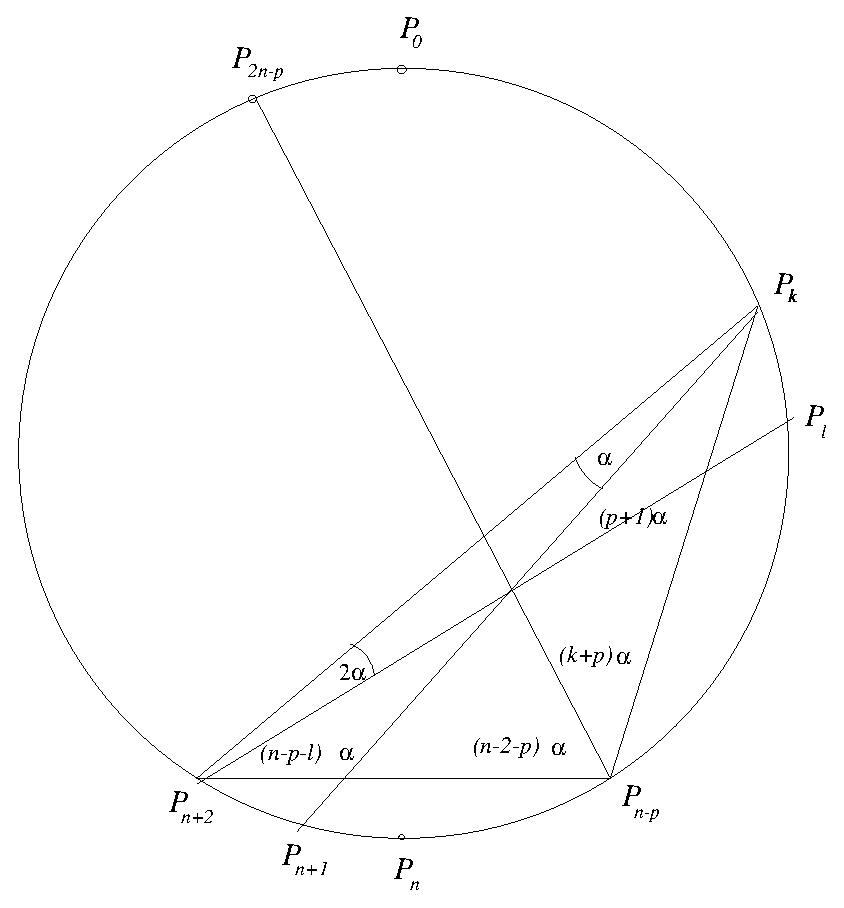
\includegraphics[width=.9\linewidth]{schueler-02-1/neck.eps}
\end{minipage}
\begin{minipage}{.5\textwidth}
Wir wenden nun diesen Satz an auf das Dreieck mit den Eckpunkten 
$A=P_{n+2}$, $B=P_{n-p}$,
$C=P_k$ und  den Ecktransversalen $AP_l$, $BP_{2n-p}$ und $CP_{n+1}$. 
Setzt man die Gr��e des Peripheriewinkels $\alpha:=\angle P_1P_nP_2$, so hat
man nach dem Peripheriewinkelsatz und mit $k=l+2$ und den obigen Bezeichnungen
\begin{xalignat*}{2}
\alpha_1&=(l-k)\alpha,&\alpha_2&=(n-p-l)\alpha,
\\
\beta_1&=(n-2-p)\alpha,&\beta_2&=(p+k)\alpha,
\\
\gamma_1&=(p+1)\alpha,&\gamma_2&=\alpha.
\end{xalignat*}
Hierbei ist $\alpha=\pi/(2n)$.
\end{minipage}

 Beachtet man die in der Aufgabe angegebenen
Werte von $k$, $l$ und $n$, so ist wegen $l-k=2$, $n-2-p=5p+7$, $n-p-l=3p+4$
und $p+k=3p+3$ die Bedingung aus dem Satz von {\sc Ceva}
�quivalent zu 
\begin{align}\label{ziel}
\sin(3p+3)\alpha{\cdot}\sin \alpha
{\cdot}\sin(3p+4)\alpha=\sin(5p+7)\alpha{\cdot}\sin(p+1)\alpha{\cdot}\sin 2\alpha.
\end{align}
Wir beweisen diese Gleichung. Wegen $\alpha=\pi/(12p+18)$ ist
$\sin (2p+3)\alpha=\sin \pi/6=1/2.  $ Also gilt 
$$2\cos\alpha\,\sin((2p+2)\alpha +\alpha)=
2\cos \alpha\,\sin(2p+3)\alpha=\cos \alpha.$$
Wendet man das Additionstheorem f�r den Sinus an sowie $1-2\sin^2x=\cos 2x$
und $2\sin x \cos x=\sin 2x$,
so hat man
\begin{align*}
2\cos^2\alpha\, \sin(2p+2)\alpha + \sin 2\alpha\,\cos(2p+2)\alpha=&\cos \alpha.
\\
2\cos^2\alpha\, \sin(2p+2)\alpha + (1- 2\sin^2(p+1)\alpha)\,\sin
2\alpha=&\cos\alpha.
\end{align*}
Subtrahiert man $\sin 2\alpha$ und beachtet erneut die Doppelwinkelformel, so
hat man
\begin{align*}
2\cos^2\alpha\, \sin(2p+2)\alpha - 2\sin^2(p+1)\alpha\,\sin 2\alpha&=
\cos\alpha-\sin 2\alpha
\\
4\cos^2\alpha\,\sin(p+1)\alpha\,\cos(p+1)\alpha-4\sin^2(p+1)\alpha\,\sin\alpha\,
\cos\alpha&=\cos\alpha-\sin
2\alpha
\\
4\cos\alpha\,\sin(p+1)\alpha\bigl(\cos(p+1)\alpha\,\cos\alpha-\sin(p+1)\alpha\,
\sin\alpha\bigr)&=\cos\alpha-\sin
2\alpha
\\
4\cos \alpha\sin(p+1)\, \alpha\cos (p+2)\alpha&=\cos\alpha-\sin
2\alpha.
\end{align*}
In der letzten Umformung benutzten wir das Additionstheorem f�r den
Kosinus. Beachtet man nun $(p+2)\alpha
+(5p+7)\alpha =2\alpha +(6p+7)\alpha=  \pi/2$ und $\sin x=\cos (\pi/2-x)$, so kann man weiter umformen
zu
\begin{align*}
4\cos \alpha\, \sin(p+1)\alpha\, \sin(5p+7)\alpha&=\cos \alpha -\cos(6p+7)\alpha
\\
4\cos \alpha\, \sin(p+1)\alpha\, \sin(5p+7)\alpha&=2\sin(3p+3)\alpha\, \sin(3p+4)\alpha,
\end{align*}
wobei wir $-\cos a +\cos b=2\sin(a+b)/2 \sin(a-b)/2$ benutzten.
Dividiert man die obige Gleichung durch $2$, multipliziert mit $\cos \alpha$
und beachtet die Doppelwinkelformel, so hat man
$$
\sin 2\alpha\, \sin(p+1)\alpha\, \sin(5p+7)\alpha=\sin
\alpha\, \sin(3p+3)\alpha\, \sin(3p+4)\alpha.
$$
Damit ist die Behauptung gezeigt; die drei Diagonalen verlaufen durch einen
Punkt.
\end{loesung}

\begin{aufgabe} (a) ({\sc Coxeter}, Unverg�ngliche Geometrie) In einem Viereck $ABCD$ sind die folgenden Winkel gegeben
$\angle BAD=\angle ABC=80 ^\circ $, $\angle ABD=50^\circ $ und $\angle
BAC=60^\circ$. Man bestimme die Gr��e des Winkels $\angle BCD$!
\\
(b) In einem Viereck $ABCD$ sind die folgenden Winkel gegeben
$\angle BAD=\angle ABC=84 ^\circ $, $\angle ABD=54^\circ $ und $\angle
BAC=66^\circ$. Man bestimme die Gr��e des Winkels $\angle BCD$!
\end{aufgabe}

\begin{loesung} (a) Wir benutzen f�r die L�sung die Aufgabe\,\ref{allg} mit
  $p=0$. Mit $p=0$ haben
  wir $n=9$, $k=3$, $l=5$, $\alpha=10 ^\circ$. Wir betten das Viereck $ABCD$
  ein in ein regul�res $18$-Eck $P_0P_1\cdots P_{17}$ mit $A=P_{10}$ und $B=P_9$. Wir zeigen, dass $D$
  der Schnittpunkt $S$  der Diagonalen $P_1P_{10}$ und $P_9P_{15}$ ist und $C$ der
  Schnittpunkt $T$ der Diagonalen $P_0P_9$, $P_3P_{10}$ und $P_5P_{11}$ ist (wegen
  Aufgabe\,\ref{allg} gehen diese 3 durch einen gemeinsamen Punkt). Aus
  Symmetriegr�nden liegt $S$ auch auf der Diagonalen $P_5P_{11}$.
\\
Klar ist, dass $\angle ABC=\angle BAD=8\alpha=80^\circ$ gilt. Ferner ist
  $\angle ABS=(15-10)\alpha=5\alpha=50^\circ$. Folglich git $D=S$. Au�erdem
  ist $\angle CAB=\angle P_3AP_{9}=6\alpha=60^\circ$. Somit ist $C=T$. Damit
  ist aber klar, dass nach Au�enwinkelsatz im Dreieck $P_5P_9C$ gilt $\angle
  BCD=\angle BP_5 P_{11}+\angle P_0BP_5=2\alpha   +5\alpha=7\alpha=70^\circ$.

(b) Wir betten das Viereck in ein regelm��iges $30$-Eck $P_0P_1\cdots P_{29}$
mit dem Mittelpunkt $Z$ ein mit $A=P_{16}$, $B=P_{15}$ , $C:=P_{4}P_{16}\cap
BZ$ und $D:=P_{15}P_{25}\cap AZ$. Es ist $\alpha=180^\circ/30=6^\circ$. Dann
ist zun�chst klar, dass  $\angle ABC=\angle BAD=14\alpha=84^\circ$
gilt. Ferner ist 
  $\angle ABD=(25-16)\alpha=9\alpha=54^\circ$ und $\angle
  CAB=(15-4)\alpha=11\alpha=66^\circ.$
\\
Wir sind fertig, wenn wir zeigen k�nnen, dass $CD\equiv P_7P_{17}$ gilt. Aus
Symmetriegr�nden ist klar, dass sich $P_7P_{17} $ und $P_5P_{25}$ auf $AZ$
schneiden. Wir zeigen nun analog zu Aufgabe\,\ref{allg}, dass sich die drei
Diagonalen $P_7P_{17}$, $P_4P_{16}$ und $P_0P_{15}$ in einem Punkt
schneiden. Mit den Bezeichnungen von Aufgabe\,\ref{allg} hat das Dreieck
$P_{17}P_{15}P_4$ hat die Winkelgr��en
\begin{xalignat*}{2}
\alpha_1&=8\alpha,&\alpha_2&=3\alpha,
\\
\beta_1&=13\alpha,&\beta_2&=4\alpha,
\\
\gamma_1&=\alpha,&\gamma_2&=\alpha.
\end{xalignat*}
Die Bedingung aus der trigonometrischen Form des Satzes von {\sc Ceva} lautet
damit
$$
\sin 8\alpha{\cdot} \sin 4\alpha=\sin 13\alpha{\cdot}\sin 3\alpha
\quad\text{bzw.{}}\quad
\sin 48^\circ \sin 24^\circ=\sin 78^\circ{\cdot}\sin 18^\circ.
$$
Dies ist aber unter Benutzung der Doppelwinkelformel f�r den Sinus und ${\sin x
=\cos (\pi/2-x)}$ �quivalent zu den folgenden Gleichungen
\begin{align*}
2\sin 48^\circ\, \sin 12^\circ\cos 12^\circ&=\cos 12^\circ\, \sin 18^\circ,
\\
2\sin48^\circ\,\sin 12^\circ&=\sin 18^\circ,
\\
-\cos 60^\circ+\cos 36^\circ&=\sin 18^\circ.
\end{align*}
In der letzten Umformung benutzten wir wieder $2\sin a\sin
b=-\cos(a+b)+\cos(a-b)$. Die letzte Gleichung gilt wegen $\cos 60^\circ=1/2$,
$\cos 36^\circ= (1+\sqrt{5})/4$ und ${\sin 18^\circ=(-1+\sqrt{5})/4}$. Die drei
Ecktransversalen schneiden sich also in einem gemeinsamen Punkt.
\\
Wir erhalten mit dem Au�enwinkelsatz im Dreieck $P_7CB$, dass
\begin{align*}
\angle BCD=\angle P_{17}P_7P_{15}+\angle
P_0P_{15}P_{7}=2\alpha+7\alpha=9\alpha=54^\circ.
\end{align*}

\end{loesung}
\begin{comment}
  todo: geometric markup
\end{comment}

\begin{attribution}
  Diese Aufgabe ist ver�ffentlicht in der WURZEL~11/02 als Aufgabe $\iota\,
  53$. Sie ist entstanden aus der L�sung der Aufgabe~2 von {\sc Coxeter}.
  Einen ausf�hrlichen Artikel �ber Mehrfachschnittpunkte in regul�ren
  $n$-Ecken findet man in

\url{http://www.mathematik.uni-bielefeld.de/~sillke/SEQUENCES/regular-n-gon.ps}

Johannes Waldmann war so freundlich, mir diesen link mitzuteilen.

Hier ist die Originalquelle:
\begin{quote}
Poonen, Bjorn; Rubinstein, Michael:
The number of intersection points made by the diagonals of a regular polygon,
{\em SIAM J. Discrete Math.} {\bf  11} (1998), no. 1, 135--156 (electronic).
\end{quote}


schueler (2004-09-14): Contributed to KoSemNet

graebe (2004-09-14): Prepared along the KoSemNet rules
\end{attribution}
\end{document}

